\documentclass[11pt]{article} 
\usepackage[english]{babel}
\usepackage[utf8]{inputenc}
\usepackage[margin=0.5in]{geometry}
\usepackage{amsmath}
\usepackage{amsthm}
\usepackage{amsfonts}
\usepackage{amssymb}
\usepackage[usenames,dvipsnames]{xcolor}
\usepackage{graphicx}
\usepackage[siunitx]{circuitikz}
\usepackage{tikz}
\usepackage{tkz-berge}
\usetikzlibrary{positioning, automata, backgrounds}
\usepackage[colorinlistoftodos, color=orange!50]{todonotes}
\usepackage{hyperref}
\usepackage[numbers, square]{natbib}
\usepackage{fancybox}
\usepackage{epsfig}
\usepackage{soul}
\usepackage[framemethod=tikz]{mdframed}
\usepackage[shortlabels]{enumitem}
\usepackage[version=4]{mhchem}
\usepackage{multicol}
\usepackage{forest}
\usepackage{mathtools}
\usepackage{comment}
\usepackage{enumitem}
\usepackage[utf8]{inputenc}
\usepackage{listings}
\usepackage{color}
\usepackage[numbers]{natbib}
\usepackage{subfiles}
\usepackage{tkz-berge}
\usepackage{algorithm}
\usepackage[noend]{algpseudocode}


\newtheorem{prop}{Proposition}[section]
\newtheorem{thm}{Theorem}[section]
\newtheorem{lemma}{Lemma}[section]
\newtheorem{cor}{Corollary}[prop]

\theoremstyle{definition}
\newtheorem{definition}{Definition}

\theoremstyle{definition}
\newtheorem{required}{Problem}

\theoremstyle{definition}
\newtheorem{ex}{Example}

\newcommand{\interval}[4]{\draw (#2, #1) -- (#3, #1); % Usage: \interval{height}{start}{end}{label}
\draw (#2, #1-0.11) -- (#2, #1+0.11); % draw left whisker
\draw (#3, #1-0.11) -- (#3, #1+0.11); % draw right whisker
\node[] at (#2-0.25, #1) {#4};
}


\setlength{\marginparwidth}{3.4cm}
%#########################################################

%To use symbols for footnotes
\renewcommand*{\thefootnote}{\fnsymbol{footnote}}
%To change footnotes back to numbers uncomment the following line
%\renewcommand*{\thefootnote}{\arabic{footnote}}

% Enable this command to adjust line spacing for inline math equations.
% \everymath{\displaystyle}

% _______ _____ _______ _      ______ 
%|__   __|_   _|__   __| |    |  ____|
%   | |    | |    | |  | |    | |__   
%   | |    | |    | |  | |    |  __|  
%   | |   _| |_   | |  | |____| |____ 
%   |_|  |_____|  |_|  |______|______|
%%%%%%%%%%%%%%%%%%%%%%%%%%%%%%%%%%%%%%%

\title{
\normalfont \normalsize 
\textsc{CSCI 3104 Fall 2021 \\ 
Instructors: Profs. Grochow and Waggoner} \\
[10pt] 
\rule{\linewidth}{0.5pt} \\[6pt] 
\huge Problem Set 9 \\
\rule{\linewidth}{2pt}  \\[10pt]
}
%\author{Your Name}
\date{}

\begin{document}
\definecolor {processblue}{cmyk}{0.96,0,0,0}
\maketitle


%%%%%%%%%%%%%%%%%%%%%%%%%
%%%%%%%%%%%%%%%%%%%%%%%%%%
%%%%%%%%%%FILL IN YOUR NAME%%%%%%%
%%%%%%%%%%AND STUDENT ID%%%%%%%%
%%%%%%%%%%%%%%%%%%%%%%%%%%
\noindent
Due Date \dotfill TODO \\
Name \dotfill \textbf{Didi Trifonova} \\
Student ID \dotfill \textbf{109388776} \\
Collaborators \dotfill \textbf{Maria Garcia}

\tableofcontents

\section{Instructions}
 \begin{itemize}
	\item The solutions \textbf{must be typed}, using proper mathematical notation. We cannot accept hand-written solutions. \href{http://ece.uprm.edu/~caceros/latex/introduction.pdf}{Here's a short intro to \LaTeX.}
	\item You should submit your work through the \textbf{class Canvas page} only. Please submit one PDF file, compiled using this \LaTeX \ template.
	\item You may not need a full page for your solutions; pagebreaks are there to help Gradescope automatically find where each problem is. Even if you do not attempt every problem, please submit this document with no fewer pages than the blank template (or Gradescope has issues with it).

	\item You are welcome and encouraged to collaborate with your classmates, as well as consult outside resources. You must \textbf{cite your sources in this document.} \textbf{Copying from any source is an Honor Code violation. Furthermore, all submissions must be in your own words and reflect your understanding of the material.} If there is any confusion about this policy, it is your responsibility to clarify before the due date. 

	\item Posting to \textbf{any} service including, but not limited to Chegg, Reddit, StackExchange, etc., for help on an assignment is a violation of the Honor Code.

	\item You \textbf{must} virtually sign the Honor Code (see Section \ref{HonorCode}). Failure to do so will result in your assignment not being graded.
\end{itemize}


\section{Honor Code (Make Sure to Virtually Sign)} \label{HonorCode}

\begin{required}
\begin{itemize}
\item My submission is in my own words and reflects my understanding of the material.
\item Any collaborations and external sources have been clearly cited in this document.
\item I have not posted to external services including, but not limited to Chegg, Reddit, StackExchange, etc.
\item I have neither copied nor provided others solutions they can copy.
\end{itemize}

%\noindent In the specified region below, clearly indicate that you have upheld the Honor Code. Then type your name. 
\end{required}

\begin{proof}[Agreed (Didi Trifonova).]
%% Typing "I agree to the above," followed by your name is sufficient.
\end{proof}


\newpage
\section{Standard 24- Dynamic Programming: Design DP Algorithms}

\begin{required}
The \textsf{Highest Reflective Subsequence} problem is defined as follows.
\begin{itemize}
\item \textsf{Instance:} A string $\omega \in \Sigma^{n}$, where $\Sigma$ is our fixed alphabet.
\item \textsf{Solution:} A subsequence $\psi \in \Sigma^{\ell}$ of $\omega$ of maximum length such that for all $i \in \{1, \ldots, \ell\}$, $\psi_{i} = \psi_{\ell - i + 1}$.
\end{itemize}


\noindent \\ The goal of this problem set is to design a dynamic programming algorithm to solve the \textsf{Highly Reflective Subsequence} problem.

\begin{enumerate}[label=(\alph*)]
\subsection{Problem 2\ref{2a}}
\item \label{2a} Let $L[i, j]$ denote the length of the highest reflective subsequence of $\omega[i, \ldots, j]$. Write down a mathematical recurrence for $L[i, j]$. Clearly justify each case.

\begin{proof}[Answer]
\textbf{base cases:}
\begin{itemize}
    \item $i<j$, then $L[i, j]=0$ and $\omega = \psi$
    \item $i=j$, then $L[i, j]=1$ and $\omega = \psi$
\end{itemize}
\begin{equation}
  L[i, j]=\begin{cases}
    2 + L[i+1][j-1] & \text{if $\omega[i]$ = $\omega[j]$ }\\
    Max(L[i][j-1], L[i+1]j) & \text{otherwise}
  \end{cases}
\end{equation}
The subproblem  would be finding the highest reflective sequence starting at $L[0,0]$ and incrementing the size of the string. In this example, $i$ and $j$ correspond to the start and end of the string we are evaluating. If we start at a length of 0, then the longest substring also would just be an empty string. A length of 1 results in a subsequence of length 1 because any single character is a reflective. As we increase the length of our string we check to see if the first and last character match. We cannot increase the length of the reflective subsequence unless we have a character on each side that can be "reflective". Therefore, if the first and last letter match, then our answer is the longest subsequence from the string that does not contain the first and last character, plus 2 to account for the new match. If there is no match with the letters then we must choose the max from the either the first $i-j$ letters or the last $i-j$ letters (total length of the string we are evaluating is $i-j+1$). 
\end{proof}



\newpage
\subsection{Problem 2\ref{2b}}
\item \label{2b} Clearly describe how to construct and fill in the lookup table. For the cell $L[i, j]$, clearly describe the sub-cases we consider, which optimal sub-case we select, and any relevant pointers that should be included in the table.

\begin{proof}[Answer] $ $\\
\begin{itemize}
    \item Create a 2d lookup table with the characters of $\omega$ on each side
    \item If $i > j$ then we fill in 0 because these are strings of length $< 1$
    \item Begin with string of length 1: $L[1,1],L[2,2]...L[i,i]$. These are all a base case and have a max subsequence of length 1. 
    \item Next evaluate strings of length 2. If the first and last character match, then $L[i,j]=2 + L[i+1][j-1]$. In this case, $L[i+1][j-1]$ represents the longest subsequence from a string of length 0, thus, $L[i,j]=2 + 0 = 2$ and our back-pointer points to $L[i+1][j-1]$. If not, then $L[i,j] = Max(L[i][j-1], L[i+1]j)$. In this case, increasing the length of the string by 1 does not increase the length of our subsequence. Therefore, we can want to carry over the maximum length from a string of $j-i$ length. The two choices we have are the strings from $i$ to $j-1$ or from $i+1$ to $j$ and we choose the one that will give us the max length. Whichever one gives us the max length is where our back-pointer points to. 
    \item Continue this recursive pattern until you reach the length of your original string. For example, if your string is of length 7 then you once again have two options: either your last two characters match or they don't. If they match then your subsequence has a length of 2 plus the max subsequence of the inner 5 characters. If they don't match then you can carry over the max subsequence from a string of length 6 (first 6 characters or last 6 characters) 
\end{itemize}
\end{proof}



\newpage
\subsection{Problem 2\ref{2c}}
\item \label{2c} Work through an example of your algorithm using the input string $\omega = \texttt{abcdeca}$. Clearly show how to recover an optimal solution using your lookup table. You may hand-draw your lookup table, but your explanation must be typed.

\begin{proof}[Answer] $ $ \\
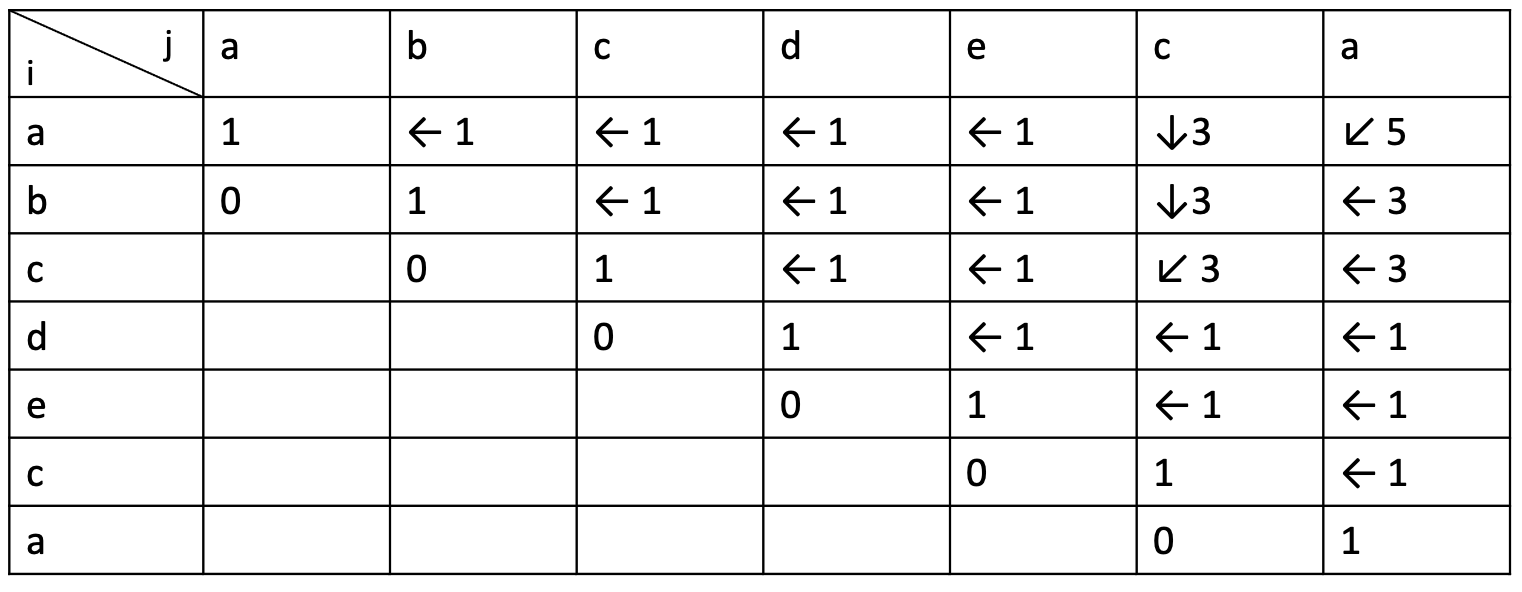
\includegraphics[width =170mm]{table2.png} \\
\begin{itemize}
    \item Fill in the base cases: strings of length 0 and 1
    \item L[1,2] $\to$ We are evalauting the string (a,b) and characters a and b do not match so we take the max from cells [1,1] or [2,2]. We do this because increasing the length to 2 will not increase the length of our subsequence so we carry over the answer from a string of length of 1. This is essentially picking between the string "a" and "b". In this case, they are both have a subsequence of length 1 and so we randomly choose [1,1] and this is what our back-pointer points to. 
    \item This pattern continues until we reach cell [3,6]. This case is different because the string we are evaluating starts with c and ends with c. This string is (c,d,e,c) and has a length of four. To find the longest reflective subsequence length we start with 2 and then we add the result from the string (d,e) which is cell [4,5]. Therefore, L[3,6] = 2 + 1 = 3 and our back-pointer points to [4,5]. 
    \item Skipping to our final cell, [1,7], we look at the case where the first and last match because our string is (a,b,c,d,e,c,a). To find our max length we start with 2 for our 2 "a" characters and we add the max length for the string (b,c,d,e,c). This corresponds to cell [2,6] which is equal to 3. Therefore, L[1,7] = 2 + 3 = 5 and our back-pointer points to [2,6]. 
    \item To recover our solution we start with our final cell and follow the back-pointers. From [1,7] we know that the first and last letters are "a". Then we follow the backpointer to [2,6] and since the letters don't match we move onto [3,6]. From here we see that "c" matches so our string becomes (a,c,c,a). We follow the back pointer again to [4,5], which doesn't match and then [4,4]. Here "d" matches and we have no more back pointers so our final string is (a,c,d,c,a) which has a length of 5, as desired. 
\end{itemize}
\end{proof}

\end{enumerate}



\end{required}

\end{document} % NOTHING AFTER THIS LINE IS PART OF THE DOCUMENT



